%!TEX TS-program = xelatex
%
% Created by Snow on 2017-11-14.
% Copyright (c) 2017 .
\documentclass{article}

\usepackage{polyglossia}
\usepackage{hyperref}
\usepackage{amsmath}
\usepackage{graphicx}
\usepackage[top=1in, bottom=1in, left=1.25in, right=1.25in]{geometry}


\newcommand{\projTitle}{SOME TITLE TO INSERT}

\title{COMP6111C Project Proposal}
\author{Authors}
\date{}

\begin{document}

\maketitle

\abstract{Abs...}

\section{Introduction}


\section{Proof-of-Statistics}
Proof-of-work has been identified as a major bottleneck of scalability of \textit{Bitcoin}  and has been tackled by replacing it with some useful work \cite{filecoin-storage} or with a new system architecture \cite{RSCoin-bank}.  Replacment of proof-of-work with some  
efficient actions in blockchain-based systems can bring a great number of benefits since the usually wasted resources aggreate to an enormous amount of  computational power \cite{bitcoin-comp-elec-power}. Cloud data centers are not an exception for such an 
improvement. Data center environements are usually highly optimized and any system resource wastage is considered as critical and intolerable \cite{google-ai-power, facebook-cold-storage-rack}. Due to such stringent data center requirements, in-data center services
shall not incur any overhead on the miners for maintaining a globally shared blockchain and shall not result in misuse of CPU or any other resource. Considering this, we propose a paradigm called 'Proof-of-Statistics', which employs the miners as ordinary computaion nodes
for performing statistical operations on received data. The CPUs and other resources are dedicated to actions that are extensively conducted in modern data centers \cite{microsoft-autopilot} and which provide the miners with a reward. 

\subsection{Data Flow and Miners}
 \textit{Bitcoin} has applied a design of a globally shared ledger for recording all the transactions occured in the system. Such a design separates two major groups: \textit{miners} and \textit{currency users}. As though, despite its architectural issues and perforamnce
problems, \textit{Bitcoin} remains a global peer-to-peer network which is used by many users every day. Thus, it appears reasonable to adhere to the original proposal of \textit{Bitcoin} and segregate \textit{minders} from \textit{clients}. The proposed system, \textit{\projTitle}, exploits the fundamental principles of \textit{Bitcoin} with an extra entity: central controller, which, in data centers, may be the administrator of the data center (Figure \ref{fig:project_design}). 
\begin{figure}[b!]
  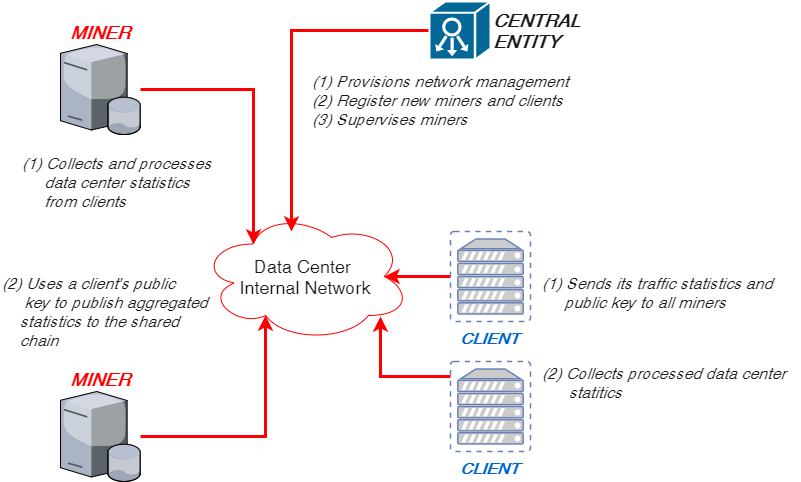
\includegraphics[width=0.65\linewidth]{project_design.png}
  \caption{Design of \textit{\projTitle}}
  \label{fig:project_design}
\end{figure}


     
\newpage
\bibliographystyle{ieeetr}
\bibliography{proposal}

\end{document}


